%-------------------------------------------------------------------------
% Design Project Input/Output Module Description
%-------------------------------------------------------------------------

\clearpage
\section{Flex Input Module}
\label{sec-input-flex}

This input module enables your IoT device to sense the flexing of a
\wu{6}{cm} strip. The flex sensor is a resistor with a resistance that
varies depending on how much the strip is flexed (e.g., by bending it);
the resistance is higher when flexed in one direction and lower when
flexed in the other. The Arduino cannot directly sense resistance, but
we can set up a voltage divider so that the Arduino can sense voltage
instead. This way, as we flex the sensor, the voltage the Arduino reads
changes accordingly.

% FIXME: replace 'ohm' with symbol..

A sample circuit and Arduino code is shown below to get you started.
The voltage divider circuit is formed by the flex sensor and the
\wu{10}{kohm} resistor, and the Arduino reads the voltage from one end
of the resistor to ground. The example code will print the analog
reading from the flex sensor on the serial monitor, similar to how we
printed the analog reading from the grayscale sensor in Lab~2. After
setting up the circuit and programming the Arduino, open the serial
monitor and check the value the flex sensor is detecting. Then try
flexing the sensor strip in either direction and see the reading
increase and decrease accordingly.

\vspace{0.1in}
\begin{minipage}[t]{0.49\tw}
  \vspace{0pt}

  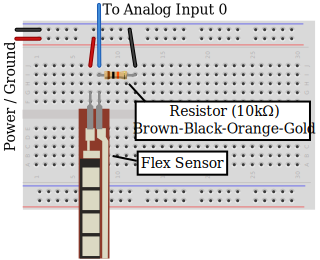
\includegraphics[width=\tw]{input-flex-annotated.svg.pdf}
\end{minipage}
\hfill
\begin{minipage}[t]{0.49\tw}
  \vspace{0.1in}
  \begin{Verbatim}[gobble=3,fontsize=\small]
    int pin_flex = A0;

    void setup() {
      Serial.begin(9600);
      pinMode( pin_flex, INPUT );
    }

    void loop() {
      int flex = analogRead( pin_flex );

      Serial.println( flex );
      delay(1000);
    }
  \end{Verbatim}
\end{minipage}
\vspace{0.1in}

%Questions:
